\begin{itemize}
    \item Grundsatz: Alles, was nicht zwingend für das Verständnis der Arbeit nötig ist, gehört in den Anhang!
\end{itemize}

\section{Project Management}
\begin{itemize}
    \item Offizielle Aufgabenstellung, Projektauftrag
    \item (Zeitplan)
    \item (Besprechungsprotokolle oder Journals)
    \item Parameters
    \item Actions
\end{itemize}

% Problem Definition (BA Ausschreibung)
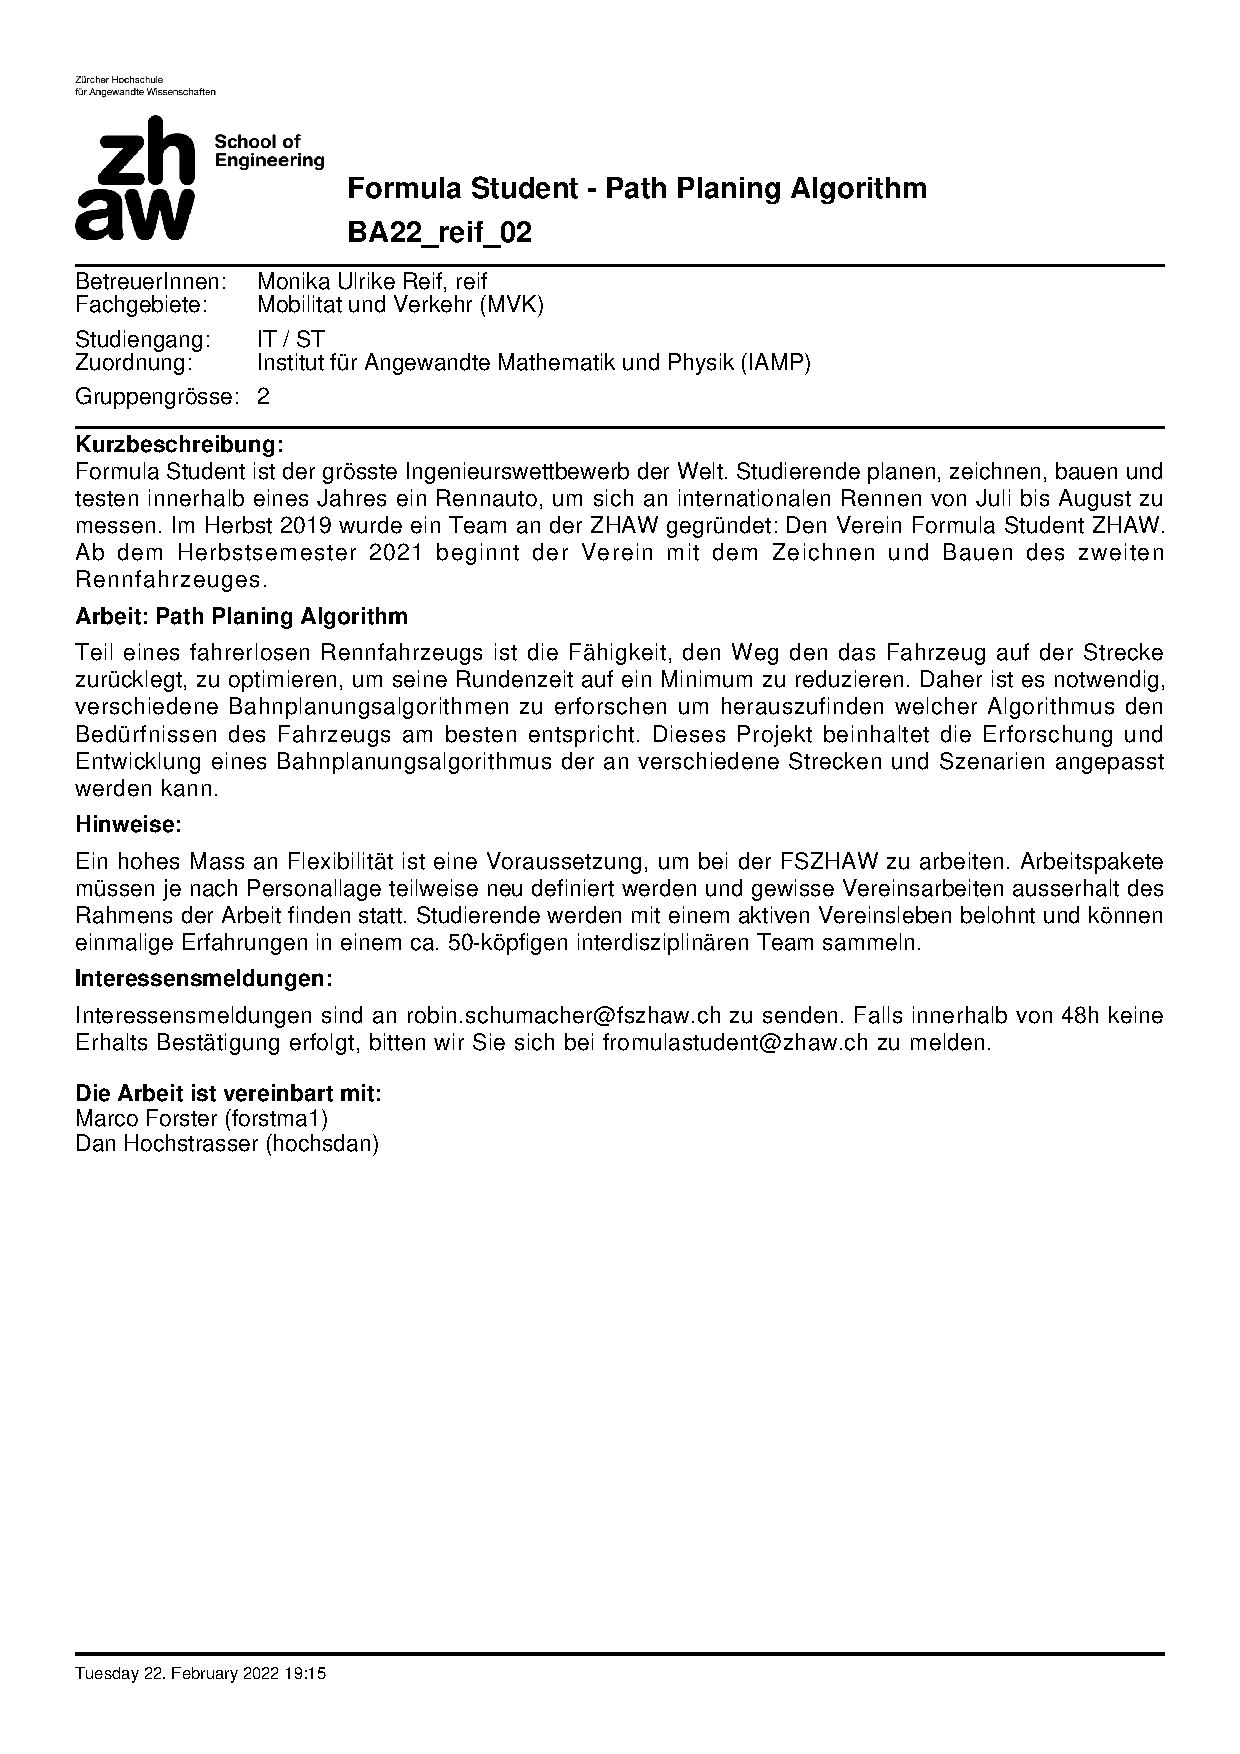
\includepdf[pages=-,pagecommand={\subsection{Problem Definition} \label{problem_definition}},width=\textwidth]{ressources/Problem_Definition}

\subsection{Path Planning Calendar Week Plan}
\begin{figure}[H]
    \centering
    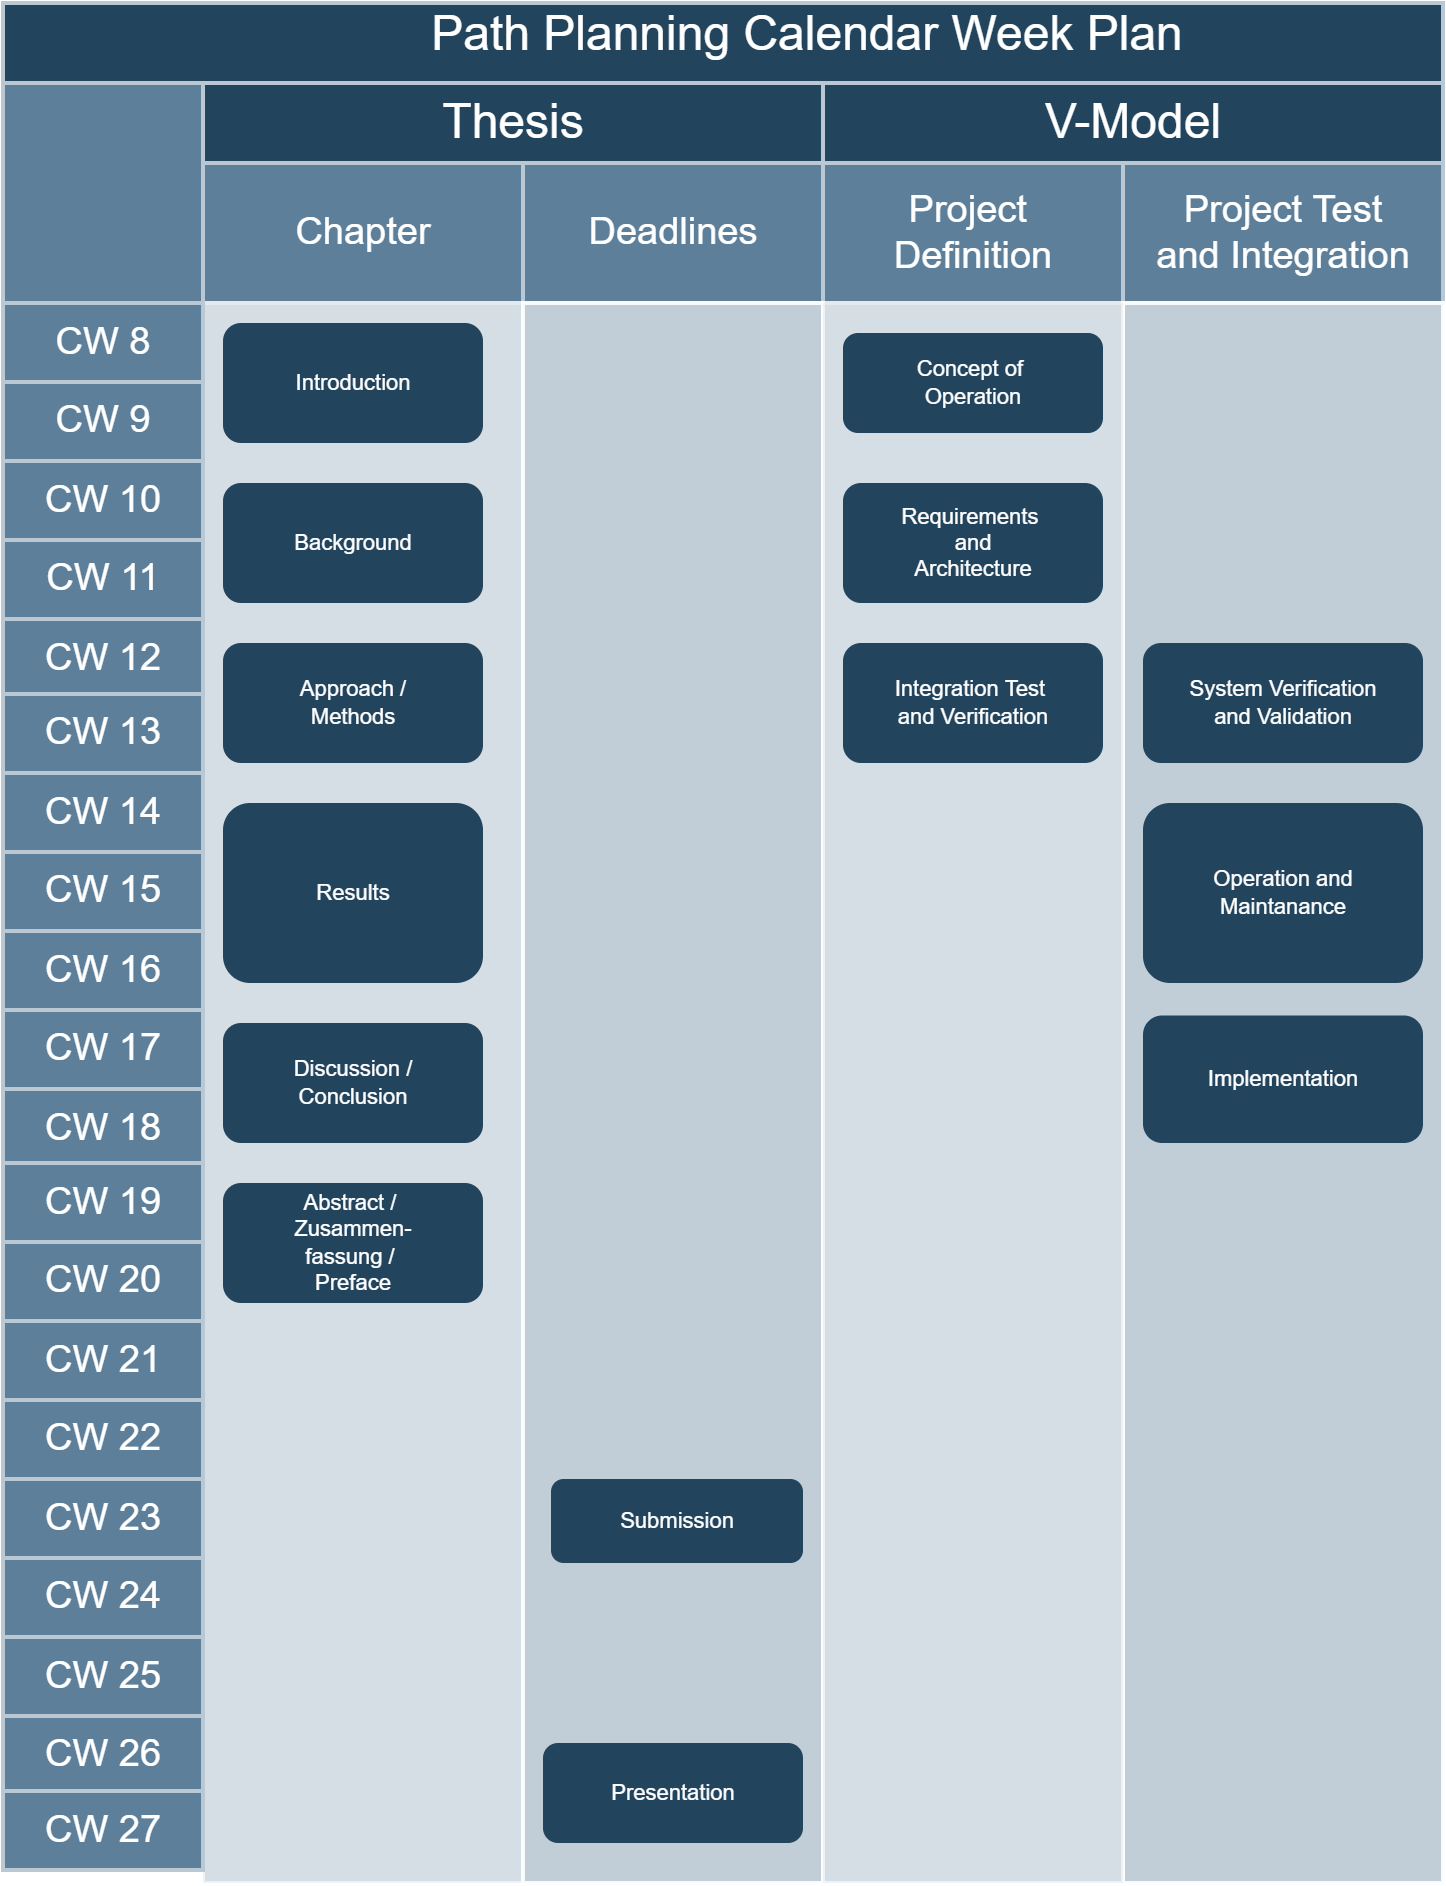
\includegraphics[width=\columnwidth]{Weekly_Plan.png}
    %\caption{The velocity space in which the car can maneuver. \cite{planning_algorithms_steven_m_lavalle}}
    \label{fig:Weekly Plan}
\end{figure}

\section{Miscellaneous}
\begin{itemize}
    \item CD mit dem vollständigen Bericht als pdf-File inklusive Daten, Film- und Fotomaterial
    \item (Schaltpläne und Ablaufschemata)
    \item (Spezifikationen u. Datenblätter der verwendeten Messgeräte und/oder Komponenten)
    \item (Berechnungen, Messwerte, Simulationsresultate)
    \item (Stoffdaten)
    \item (Fehlerrechnungen mit Messunsicherheiten)
    \item (Grafische Darstellungen, Fotos)
    \item (Datenträger mit weiteren Daten (zum Bsp. Software-Komponenten) inkl. Verzeichnis der auf diesem Datenträger abgelegten Dateien)
    \item (Softwarecode)
\end{itemize}

% FS Rules 2022 Handbook
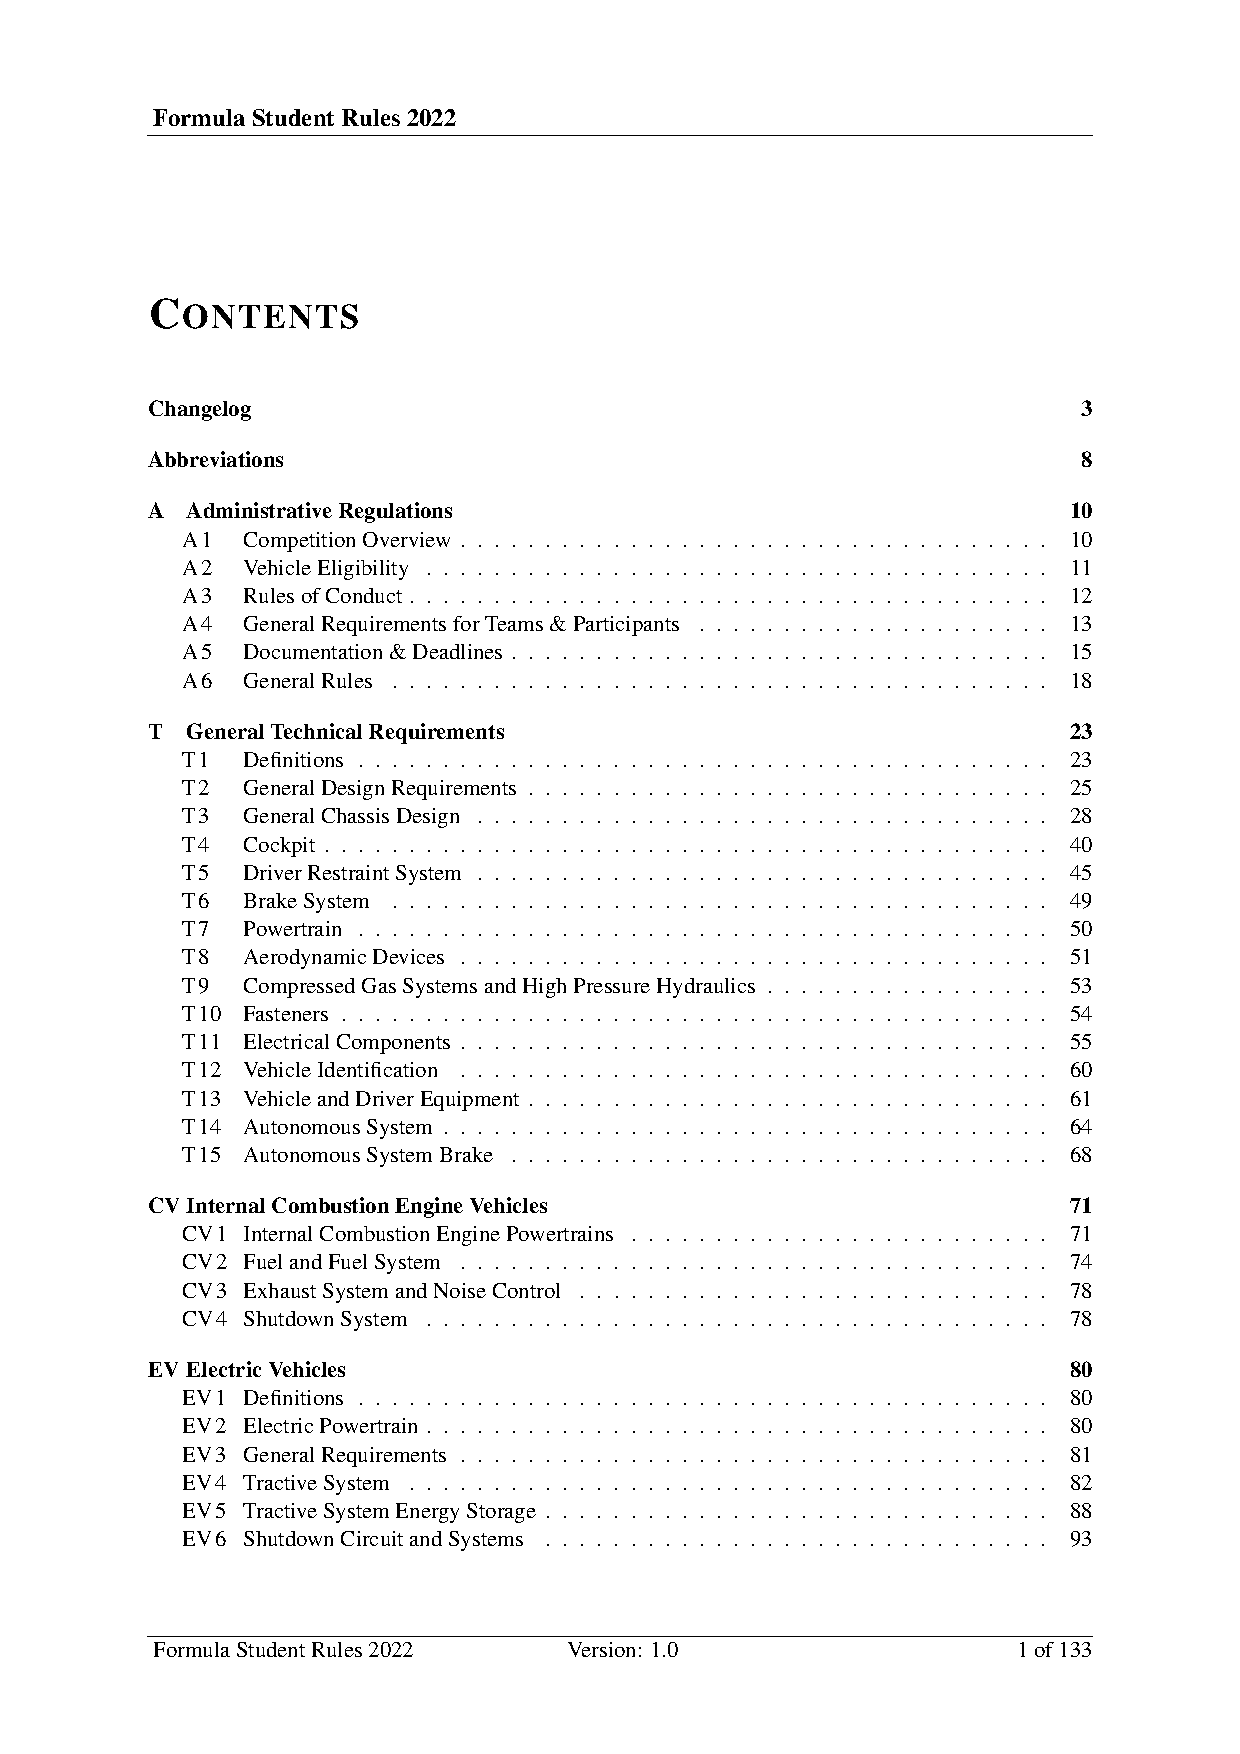
\includepdf[pages=1,pagecommand={\subsection{FS Rules 2022 Handbook} \label{fs_rules_2022_handbook}},width=\textwidth]{ressources/FS_Rules_2022_Handbook}
%\includepdf[pages=2-,pagecommand={},width=\textwidth]{ressources/FS_Rules_2022_Handbook}
% Uncomment to display all sites

\section{Scrum} \label{sec:Scrum}
Scrum is a framework which can be used by people, teams and organizations to solve problems through adaptive solutions. Four simple steps describe the process of Scrum which is lead by a Scrum Master:
\begin{enumerate}
    \item The Product Owner orders the work for a problem and puts it into a Product Backlog.
    \item The Scrum Team selects certain tasks from the Backlog, gives a number based on a certain expense and tries to realize it in a Sprint.
    \item The Scrum Team and stakeholders analyse the result and adjust it for the next sprint.
    \item After this the above steps will be repeated.
\end{enumerate}

These simplified steps help to explain how Scrum works. Scrum consists of several team roles which made up the Scrum Team. Scrum Events define what has to be done in each type of meeting. The figure \ref{fig:Scrum Framework} shows the Scrum Framework and gives an overview of the Events and Artefacts of Scrum. \cite{scrum_guide}


\begin{figure}[H]
    \centering
    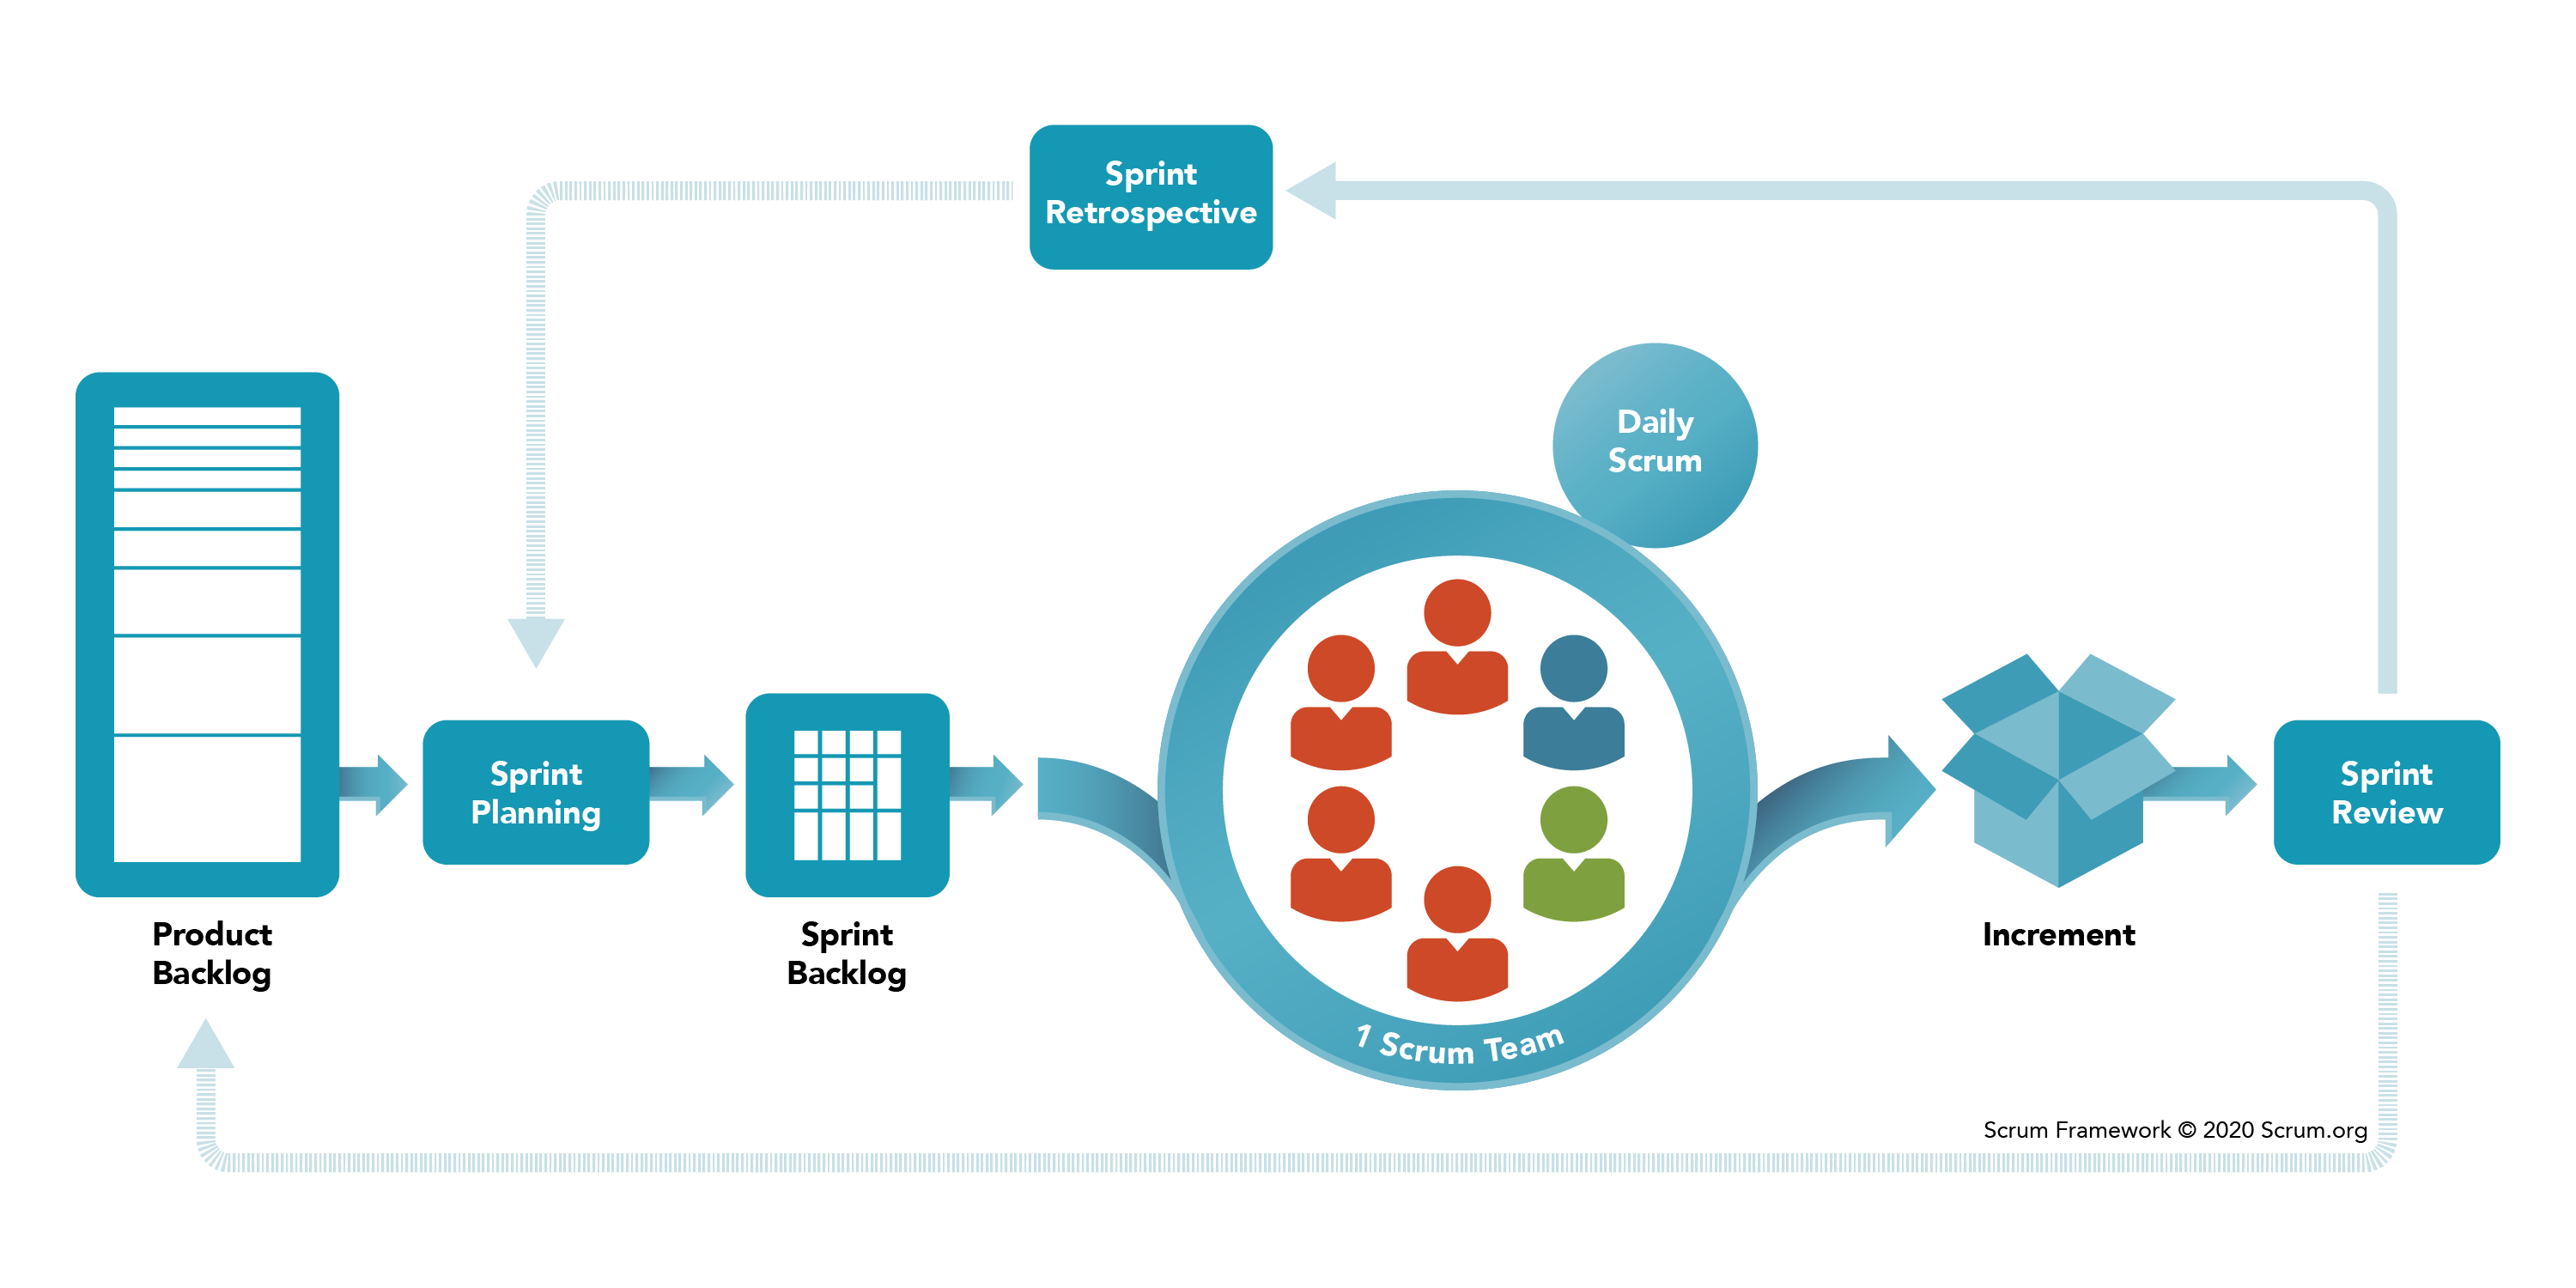
\includegraphics[width=\columnwidth]{Scrumorg_Scrum_Framework.png}
    \caption{The Scrum Framework starts with the Product Backlog and will give through the Sprint Planning certain tasks to the Sprint Backlog. The developers in the Scrum Team work on the tasks in a Sprint and define the Increment of each Sprint. After the Sprint is finished a Sprint Review will be made. \cite{scrum_guide}}
    \label{fig:Scrum Framework}
\end{figure}


\subsection{Scrum Team} \label{sec:Scrum Team}
The Scrum Team consists of one Scrum Master, a Product Owner and Developers. Normally a Scrum Team has 10 or fewer people. There are other methods to plan like Scrum on a corporate or with large amount of peoples. If the team gets to large they should consider splitting the team in smaller ones. Bellow are all the team roles with the task their doing in a Scrum Team. \cite{scrum_guide}

\textbf{Developers} are the people that create the product. Several skills are needed to work as a developer. For the Scrum specific skills they have to create a plan for the Sprint which is called the Sprint Backlog. Furthermore, they have to create methods to maintain the quality to be sure what 'Done' means in a Sprint. Next they have to adapt their plan every day until the Sprint Goal is reached. One of the most important tasks for developers is to hold themselves accountable on a professional level. \cite{scrum_guide}

\textbf{Product Owner} is responsible for the Product Backlog. The tasks of a Product Owner consist of explicitly communication the Product Goal, to create and communicate each item in the Product Backlog, orders the Product Backlog items and checks if the Product Backlog is understood by every team member. \cite{scrum_guide} The Product Owner can be a working college or an employer from another firm.

\textbf{Scrum Master} is the role where the person ensures that all members are following the Scrum Guide. The theory and practices has to be understood by every member. Self-management and cross-functionality are the abilities that the Scrum Master coaches on the team. The Scrum Master helps the developers to define 'Done' in each Sprint and ensures that every Scrum Event is held within the time frame. In terms of the Product Owner the Scrum Master helps to define the Product Goal and Backlog and serves as a middle man between the Product Owner and the developers so that everything is understood. Furthermore, he collaborates with the stakeholders if there are any requests or needs. In the Organization a Scrum Master is responsible to get employers trained on Scrum, planning and advise the implementation, makes sure that everyone understand how Scrum works and removes walls between stakeholders and the Scrum Teams. \cite{scrum_guide}

\subsection{Scrum Events} \label{sec:Scrum Events}
Scrum has so-called Scrum Events that are minimizing the need for regular meetings and to focus on transparency. The events are as followed:
\textbf{The Sprint} is the foundation of Scrum. They are normally held once a month or less. The durance of a Sprint durance is as long until another Sprint starts. In a Sprint the Product Goal, Sprint Planning, Daily Scrums, the Sprint Review and the Retrospective will be defined. During the Sprint it is not allowed to make any changes on the Sprint Goal so that the quality is not decreasing. The Product Backlog can be refined, and the scope can be adjusted. \cite{scrum_guide}

\textbf{Sprint Planning} In the sprint planning the following questions will be answered: Why is this Sprint valuable? What can be done this Sprint? How will the chosen work get done? One of the roles should be able to answer the questions. \cite{scrum_guide}

\textbf{Daily Scrum} should be a 15-minute meeting where every developer provides the current status of his task. It helps to improve communication and helps in decision-making. \cite{scrum_guide}

\textbf{Sprint Review} covers the focus on the outcome of a sprint. The team shows the progress to the stakeholders. \cite{scrum_guide}

\textbf{Sprint Retrospective} helps to improve the quality of a Sprint. The Scrum Team critics what went wrong and find solutions to improve it. \cite{scrum_guide}

\subsection{Scrum Artefacts} \label{sec:Scrum Artefacts}

Artefacts define what work has to be done. To ensure transparency commitments are defined. The commitment for the Product Backlog is the Product Goal, for the Sprint Backlog it is the Sprint Goal and for the Increment it is the definition of 'Done'. Further explanations on the different artefacts are as followed: \cite{scrum_guide}

\textbf{Product Backlog} is a list of items that can be transferred to the Sprint Backlog. The items can be a task or a number of tasks that have to be done. Each item have a 'size' that define the hours which have to be invested to finish the task. \cite{scrum_guide}

\textbf{Sprint Backlog} is a list of items which have to be worked on for the current sprint to accomplish the Sprint Goal. \cite{scrum_guide}

\textbf{Increment} is a step to the Product Goal direction. The increments are named like that because they are additive to previous increments. The Definition of 'Done' defines the state of the Increment so that the requirements of that Increment is met. \cite{scrum_guide}